%% LyX 2.0.5.1 c	reated this file.  For more info, see http://www.lyx.org/.
%% Do not edit unless you really know what you are doing.
\documentclass[11pt,oneside,final]{fithesis2}
%\usepackage[total={30em	,23cm}, includefoot]{geometry}

%% Basic packages
\usepackage[czech]{babel}
\usepackage{cmap}
\usepackage[T1]{fontenc}
\usepackage{lmodern}
\usepackage[utf8]{inputenc}
\usepackage{graphicx}

%% Additional packages for colors, advanced
%% formatting options, etc.
\usepackage{color}
\usepackage{microtype}
\usepackage{url}
\usepackage{cslatexquotes}
\usepackage{fancyvrb}
\usepackage[small,bf]{caption}
\usepackage[plainpages=false,pdfpagelabels,unicode]{hyperref}
\usepackage[all]{hypcap}

\languageattribute{czech}{split}
\usepackage{cite}
\setcounter{secnumdepth}{3}
\setcounter{tocdepth}{3}
\usepackage{hanging}
\usepackage{listings}
\usepackage{comment}
\usepackage{textcomp}
\definecolor{listinggray}{gray}{0.9}
\definecolor{lbcolor}{rgb}{0.9,0.9,0.9}
\usepackage{zref-user}
\renewcommand{\baselinestretch}{1.13}

\newcommand\todo[1]{\noindent\textcolor{red}{#1}}
\newcommand\nove[1]{\textcolor{green}{#1}}

\makeatletter
\renewcommand{\@chapapp}{}% Not necessary...
\newenvironment{chapquote}[2][2em]
  {\setlength{\@tempdima}{#1}%
   \def\chapquote@author{#2}%
   \parshape 1 \@tempdima \dimexpr\textwidth-2\@tempdima\relax%
   \itshape}
  {\par\normalfont\hfill--\ \chapquote@author\hspace*{\@tempdima}\par\bigskip}
\makeatother

%% Fix long URLs in DVIs
\usepackage{ifpdf}
\ifpdf
\else
  \usepackage{breakurl}
\fi

%% Packages used to generate various lists
\usepackage{makeidx}
\makeindex

\usepackage[xindy]{glossaries}
\makeglossary
 
\thesistitle{Srovnání RAD~platforem Seam~Forge a~Spring~Roo} % enter thesis title
\thesissubtitle{Bakalářská práce}
\thesisstudent{Jan Holman} % name of the author
\thesiswoman{false} % defines author’s gender
\thesisuniversity{Masarykova univerzita}
\thesisfaculty{Fakulta informatiky}
\thesislogo{fi-logo}
\thesisyear{Brno, jaro 2013}
\thesisadvisor{Mgr. Marek Grác, Ph.D.} % fill in advisor’s name
\thesislang{cs} % thesis is in Czech

%% Beginning of the document
\begin{document}

%% Front page with a logo and basic thesis information
\FrontMatter
\ThesisTitlePage

%% Thesis declaration (required)
\begin{ThesisDeclaration}
  \DeclarationText
  \AdvisorName
\end{ThesisDeclaration}


%% Thanks (optional)
\begin{ThesisThanks}

\end{ThesisThanks}


%% Abstract (required)
\begin{ThesisAbstract}

\end{ThesisAbstract}

%% Keywords (required)
\begin{ThesisKeyWords}

\end{ThesisKeyWords}

%% Beginning of the thesis itself
\MainMatter

%% TOC (required)
\tableofcontents

%% Thesis text structured using
%% chapters, sections, subsections, etc.
\chapter{Úvod} 
\section{Cíle práce}
\section{Struktura práce}

\chapter{Rapid Application Development}
\begin{chapquote}{The Mustard Seed Garden Manual of Painting}
Some consider it noble to have a method; others consider it noble 
not to have a method. Not to have a method is bad; to stop entirely 
at method is still worse. One should at first observe rules severely, 
then change them in an intelligent way. The aim of possessing 
method is to seem finally as if one had no method.
\end{chapquote}

Rapid Application Development, v překladu \uv{rychlý vývoj aplikací} je metodologie tvorby (mj.) softwaru, která, jak už název napovídá, upřednostňuje rychlost vytváření funkčních prototypů tradičně na úkor použitelnosti, rozsahu implementovaných funkcí a / nebo výkonu. RAD také značně omezuje část plánování ve prospěch samotného vývoje, který probíhá iterativně. Důraz se klade na tvorbu prototypů, na aktivní komunikaci s klientem a jeho participaci na vývoji \todo{citace}. Metoda byla poprvé popsána v roce 1991 Jamesem Martinem v knize Rapid Application Development jako reakce na tehdejší metody vývoje, které zejména nedokázaly dostatečně pružně reagovat na změny požadavků v průběhu vývoje, a na základě potřeby dodat co nejrychleji fungující systém.\cite{BlueInk} 

\section{Rozdíly oproti jiným metodám}
Hlavní problém tehdy nejrozšířenější metody tzv. vodopádu je ten, že vývoj systému trvá příliš dlouho. V průběhu vleklého vývoje se mohou klientovy potřeby změnit, takže výsledkem je sice kompletní a technicky dokonalý ale zároveň nepoužitelný systém. Čím déle vývoj trvá, tím vyšší je pravděpodobnost změny v požadavcích, a na tyto změny je třeba pružně reagovat.
Oproti běžným agilním metodám se RAD soustředí na vývoj pro uživatele nejzajímavějších částí \todo{(?)} – vychází z předpokladu, že uživatelé nejčastěji využívají funkce, které jsou pro ně zajímavé, a proto mají tyto části vyšší prioritu. \todo{citace} RAD také klade důraz na co nejrychlejší naplnění potřeby klienta, spíš než na technickou a technologickou dokonalost. 
Hlavní oblasti, ze kterých plyne rychlost vývoje pomocí RAD jsou prototypování, iterace a tzv. timeboxing.\\
Prototypování spočívá v co možná nejrychlejší vytvoření fungujícího prototypu (řádově v jednotkách dní), který se zaměřuje pouze na klíčové funkce, a v jeho následném ladění na základě odezvy od klienta a budoucích uživatelů. Nejde pouze o jednorázové prototypy, jako u jiných agilních metod (\todo{např.}), celý software vzniká iterativně postupným rozšiřováním prvotního prototypu. Prototyp slouží jako důkaz práce pro klienta (například při vývoji pomocí vodopádu klient velmi dlouho nevidí žádný nebo minimální výstup) a také jako referenční bod, ze kterého se vychází při dalším zpřesňování požadavků. Rychlé tvorby prvního prototypu se dosahuje využíváním tzv. CASE \todo{odkaz dolů} nástrojů, které z formálního zápisu požadavků automaticky generují datový model, funkční databázi a aplikační kód.\\
Podle pravidla timeboxingu je nutné dodávat výsledky každé iterace včas, a to i za cenu, že se část nestihne a přesune se do dalšího cyklu. Je lepší dodat část zadání včas, než dodat všechno, ale nedodržet časový plán. Pokud by se jednotlivé cykly protahovaly, omezovala by se odezva od klienta a metoda by tím ztrácela podstatnou část výhod z plynoucích z iterativního vývoje.\\
Během vytváření modelu i celého iteračního procesu jsou také aktivně zapojeni uživatelé/klient, kteří se podílejí na návrhu a schvalují prototypy. 

\section{Fáze vývoje pomocí RAD}
\begin{figure}[h!]
  \centering
    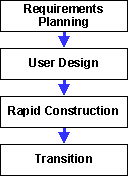
\includegraphics[scale=0.4]{img/rad-phases.png}
    \caption{Fáze RAD\cite{RAD1}}
\end{figure}

\begin{enumerate}
\item Plánování požadavků: Definování funkcí, procesů, dat a rozsahu sytému. Výsledkem je seznam entit a diagramů, které definují interakce mezi procesy a datovými elementy. Zachycení požadavků v nástroji tak, aby se daly později automaticky převést na datový model a kód (ne pouze v nestrukturovaném dokumentu).
\item Uživatelský návrh: Workshopy s uživateli/klientem, modelování dat a procesů systému, vytvoření funkčního prototypu kritických částí systému. Detailní rozvedení požadavků a převedení definovaných entit na datový model, formalizování pravidel, tvorba testovacích plánů, návrh obrazovek uživatelského rozhraní a vazeb mezi nimi. Odhad náročnosti vývoje daného systému, vytvoření prvního omezeného prototypu, který se zaměřuje pouze na (předem definované) klíčové funkce, pomocí CASE nástrojů.
\item Rychlý vývoj: Vlastní tvorba samotného aplikačního systému, tvorba uživatelské podpory a implementace pracovních plánů. Vývoj probíhá v krátkých cyklech - vývoj, testování, upřesnění požadavků, další cyklus (s využitím principu timeboxingu). Převod datového modelu na funkční databázi. 
\item Nasazení: Akceptační testování, školení uživatelů, konverze dat, nasazení systému do podniku.\cite{RAD-pdf}
\end{enumerate}

\section{Výhody}
Hlavní výhody plynoucí z RAD jsou rychlost a kvalita. Rychlost je zde dána krátkou dobou mezi dodávkami v jednotlivých cyklech, především díky využívání CASE nástrojů, které ve velmi krátkém čase konvertují požadavky na kód, a principu timeboxingu, tedy striktního dodržování časového plánu. Kvalita se v případě RAD nechápe v tradičním (a asi intuitivnějším) významu, tedy ve smyslu míry, do jaké výsledný systém splňuje zadané požadavky, a míry, do jaké v něm po dodání nedochází k závadám, ale spíš se chápe jako míra, do jaké systém naplňuje potřeby klienta a do jaké má malé náklady na údržbu. Vysoké kvality se v případě RAD dosahuje pomocí aktivního zapojené budoucích uživatelů do celého procesu tvorby systému, především ve fázích analýzy a návrhu.\cite{BlueInk}

\section{Nevýhody}
Problémy, které mohou při vývoji pomocí RAD potenciálně vzniknout, jsou především horší škálovatelnost a omezený rozsah vytvořeného systému. Protože při vývoji nejprve vzniká jednoduchý prototyp, který se později iterativně rozvíjí do kompletní aplikace, může výsledek škálovat hůř, než řešení, které je od počátku navržené jako kompletní aplikace.
Výsledná aplikace může také vlivem timeboxingu, tedy upřednostňováním včasného doručení před implementováním všech slíbených funkcí, obsahovat méně funkcí, než aplikace vytvořená tradičním způsobem (například metodou vodopádu).\\
RAD se samozřejmě nedá použít na všechny typy projektů – například systém řízení letadla vytvořený pomocí RAD by asi moc důvěry nevzbuzoval. Tento přístup je vhodný zejména pro menší projekty, nebo pro projekty, u kterých lze práci rozdělit na více zvládnutelných částí. Stejně tak by měl být poměrně malý i vývojářský tým (ideálně 2-6 lidí) a jeho členové by s tímto typem vývoje měli mít zkušenosti. Nutnou podmínkou jsou dobře definované požadavky a rozsah vytvářené aplikace, malé množství rozhodujících na straně klienta (ideálně 1 člověk) a jejich jasně určení.\cite{BlueInk} 

\section{Nástroje podporující metodu RAD}
Důležitou součástí vývoje pomocí RAD je využívání kvalitních nástrojů podporujících rychlý vývoj, tedy především CASE nástrojů, které generují aplikační kód. Bohužel ne všechny nástroje, které o sobě prohlašují, že podporují rychlý vývoj, jsou pro metodu RAD skutečně vhodné. Použité nástroje by měly umět strukturovaně zachytit požadavky (UML \todo{odkaz dolů} nástroje), převést zachycené požadavky na datový model a na jeho základě vygenerovat funkční databázi a velkou část aplikačního kódu.\\
Základní požadavky na kvalitní nástroj podporující RAD\cite{BlueInk} :
\begin{itemize}
  \item produkuje kód na úrovni enterprise (n-tier) \todo{?}
  \item generuje kompletní prvotní prototyp bez nutnosti přímého psaní kódu (vč. prezentační vrstvy)
  \item umožňuje plnou kontrolu nad generovaným kódem, například pomocí šablon
  \item poskytuje flexibilní systém metadat \todo{?}
  \item dá se použít během celého vývoje a zejména nepřepíše kód vývojáře
\end{itemize}

\url{http://en.wikipedia.org/wiki/List_of_graphical_user_interface_builders_and_rapid_application_development_tools}

\section{Spring Roo}
\subsection{Rozšíření}

\section{JBoss Forge}
\subsection{Rozšíření}

\section{Rozdíly}

\chapter{Testování UI webových aplikací}

\section{Selenium}	
\subsection{Selenium Remote Control}
\subsection{Selenium Grid}
\subsection{Selenium WebDriver}

\section{Arquillian Drone}	

\section{Arquillian Graphene 2}

\chapter{Vlastní tvorba pluginů}
\section{Plugin pro JBoss Forge}
\subsection{Použité nástroje}

\section{Addon pro Spring Roo}
\subsection{Použité nástroje}

\chapter{Závěr}

%% Lists of tables and figures, glossary, etc.
\printindex
\printglossary
\listoffigures
\listoftables


\begin{thebibliography}{13}

\bibitem{RAD1}
\textit{Článek o RAD.} [online]. [2012] [cit. 2013-12-17]. Dostupné~z:
\url{http://www.projectmanagement.com/content/processes/11306.cfm}

\bibitem{RAD-pdf}
\textit{Slidy k přednášce o RAD.} [online]. [2012] [cit. 2013-12-17]. Dostupné~z:
\url{http://www.ftms.edu.my/pdf/Download/PostgraduateStudent/IMM006%20RAPID%20APPLICATION%20DEVELOPMENT%20-%20Power%20Point%20Slide%20chapter%201.pdf}

\bibitem{BlueInk}
\textit{Článek o RAD.} [online]. [2012] [cit. 2013-12-17]. Dostupné~z:
\url{http://www.blueink.biz/RapidApplicationDevelopment.aspx}

\end{thebibliography}

%% Additional materials
\appendix

%% End of the whole document
\end{document}
